\documentclass{beamer}
\usepackage{tikz}
\usetheme{Berlin}
\newcommand{\ju}{{\scriptsize m USD }}
\renewcommand{\arraystretch}{1.5}
\title{Asset Classes}
\begin{document}
    \maketitle

%-------------------------------------------------------------------------%
% overview
%-------------------------------------------------------------------------%
\section{Overview}

\begin{frame}{Cash vs. Bonds vs. Stocks: An Asset-Based Perspective}
	\begin{itemize}
		\item Remember that \underline{assets} produce something of value, while \underline{securities} are claims to the output of the asset
		\item The value of a firm's assets is uncertain, and depends on how well the firm performs, the state of the economy, and so on
		\item Suppose an investor's portfolio contains some cash, some of the firm's bonds, and some of its stock
		\item How does the value of her portfolio vary with the value of the firm's assets?
	\end{itemize}
\end{frame}

\iffalse
\begin{frame}{Cash vs. Bonds vs. Stocks: An Asset-Based Perspective}
	\begin{center}
		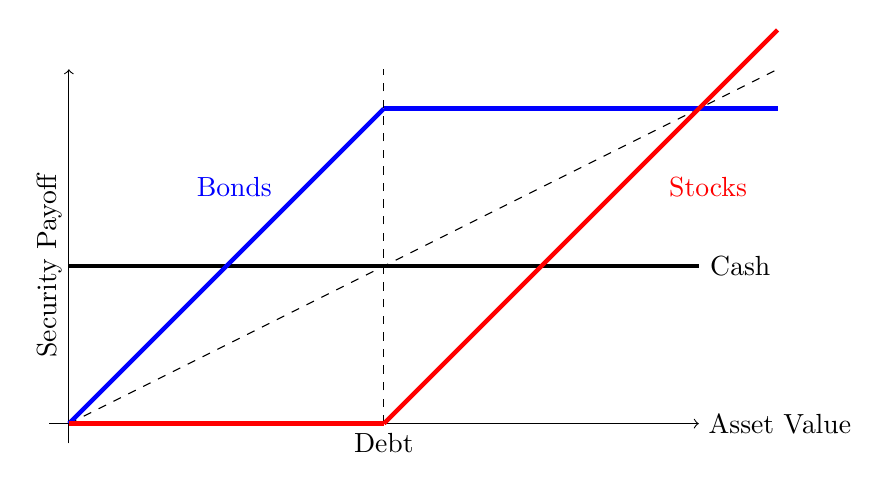
\begin{tikzpicture}
			\draw[->] (-.25,0) -- (8,0) node[anchor=west]{Asset Value};
			\draw[->] (0,-.25) -- (0,4.5);
			\draw[dashed] (4,0) node[anchor=north]{Debt} -- (4,4.5);
			\draw[dashed] (0,0) -- (9,4.5);
			\draw (-.25,2) node[rotate=90]{Security Payoff};
			% cash
			\draw[ultra thick] (0,2) -- (8,2) node[anchor=west]{Cash};
			% bonds
			\draw[ultra thick,color=blue] (0,0) -- (4,4);
			\draw[ultra thick,color=blue] (4,4) -- (9,4);
			\draw (1.5,3) node[anchor=west]{\color{blue}Bonds};
			% stocks
			\draw[ultra thick,color=red] (0,0) -- (4,0);
			\draw[ultra thick,color=red] (4,0) -- (9,5);
			\draw (7.5,3) node[anchor=west]{\color{red}Stocks};
		\end{tikzpicture}
	\end{center}
\end{frame}
\begin{frame}{Example}
	\begin{itemize}
			\item The investor has a cash balance of 10\ju and owns 40\% of the firm's stock and 60\% of its bonds
			\item The firm owes 50\ju (principal and interest) to bondholders and its asset are worth 75\ju
			\item How much is her portfolio worth?
	\end{itemize}
\end{frame}
\fi
\begin{frame}{Cash vs. Bonds vs. Stocks: An Asset-Based Perspective}
	\begin{center}
		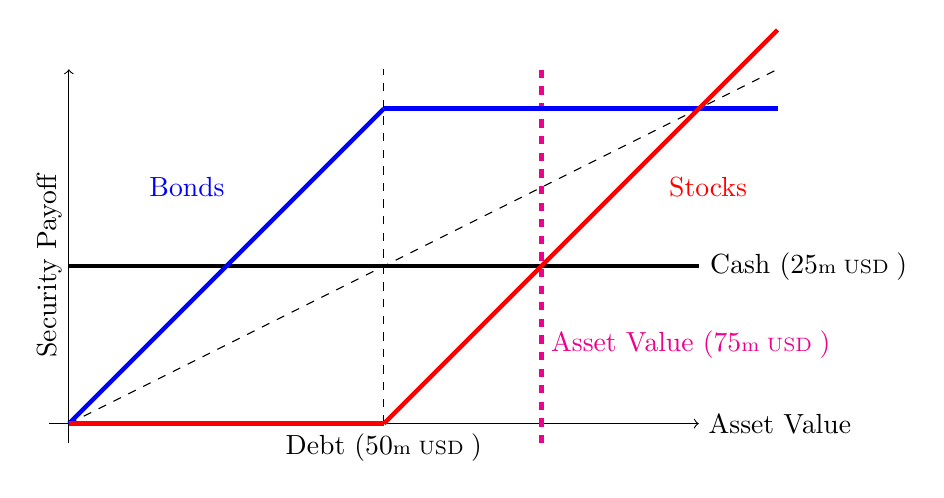
\begin{tikzpicture}
			\draw[->] (-.25,0) -- (8,0) node[anchor=west]{Asset Value};
			\draw[->] (0,-.25) -- (0,4.5);
			\draw[dashed] (4,0) node[anchor=north]{Debt (50\ju)} -- (4,4.5);
			\draw[dashed] (0,0) -- (9,4.5);
			\draw (-.25,2) node[rotate=90]{Security Payoff};
			% asset value
			\draw[dashed,ultra thick,color=magenta] (6,-.25) -- (6,4.5);
			\draw (6,1) node[anchor=west]{\color{magenta}Asset Value (75\ju)};
			% cash
			\draw[ultra thick] (0,2) -- (8,2) node[anchor=west]{Cash (25\ju)};
			% bonds
			\draw[ultra thick,color=blue] (0,0) -- (4,4);
			\draw[ultra thick,color=blue] (4,4) -- (9,4);
			\draw (1.5,3) node{\color{blue}Bonds};
			% stocks
			\draw[ultra thick,color=red] (0,0) -- (4,0);
			\draw[ultra thick,color=red] (4,0) -- (9,5);
			\draw (7.5,3) node[anchor=west]{\color{red}Stocks};
		\end{tikzpicture}
	\end{center}
\end{frame}
\iffalse
\begin{frame}{Example}
	\begin{itemize}
			\item The firm pays 50\ju to bondholders, and the remaining 25\ju to stockholders
			\item The investor keeps her cash balance of 10\ju and receives 60\%$\times$50\ju$=$30\ju from the firm's bonds and 40\%$\times$25\ju$=$10\ju from the firm's stock
			\item Her portfolio is worth 50\ju
	\end{itemize}
\end{frame}

\begin{frame}{Example}
	\begin{itemize}
			\item The investor has a cash balance of 10\ju and owns 40\% of the firm's stock and 60\% of its bonds
			\item The firm owes 50\ju (principal and interest) to bondholders and its asset are worth 25\ju
			\item How much is her portfolio worth?
	\end{itemize}
\end{frame}
\fi

\begin{frame}{Cash vs. Bonds vs. Stocks: An Asset-Based Perspective}
	\begin{center}
		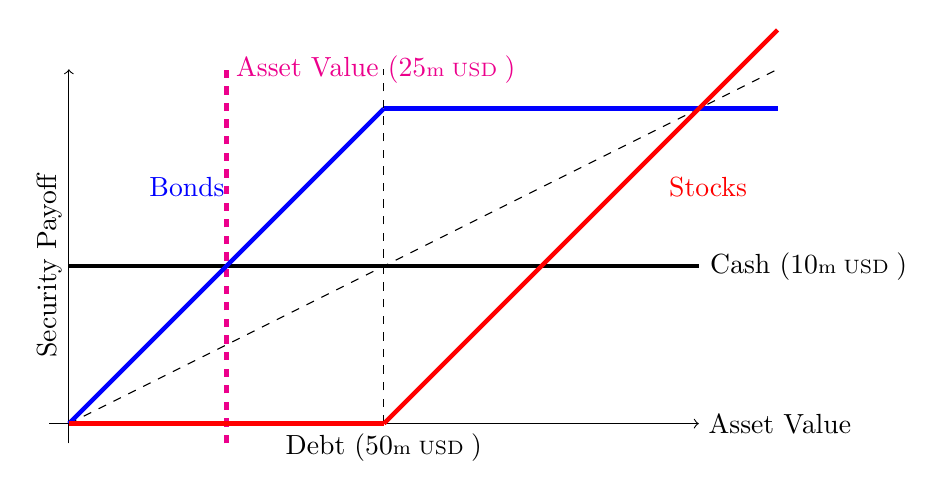
\begin{tikzpicture}
			\draw[->] (-.25,0) -- (8,0) node[anchor=west]{Asset Value};
			\draw[->] (0,-.25) -- (0,4.5);
			\draw[dashed] (4,0) node[anchor=north]{Debt (50\ju)} -- (4,4.5);
			\draw[dashed] (0,0) -- (9,4.5);
			\draw (-.25,2) node[rotate=90]{Security Payoff};
			% asset value
			\draw[dashed,ultra thick,color=magenta] (2,-.25) -- (2,4.5);
			\draw (2,4.5) node[anchor=west]{\color{magenta}Asset Value (25\ju)};
			% cash
			\draw[ultra thick] (0,2) -- (8,2) node[anchor=west]{Cash (10\ju)};
			% bonds
			\draw[ultra thick,color=blue] (0,0) -- (4,4);
			\draw[ultra thick,color=blue] (4,4) -- (9,4);
			\draw (1.5,3) node{\color{blue}Bonds};
			% stocks
			\draw[ultra thick,color=red] (0,0) -- (4,0);
			\draw[ultra thick,color=red] (4,0) -- (9,5);
			\draw (7.5,3) node[anchor=west]{\color{red}Stocks};
		\end{tikzpicture}
	\end{center}
\end{frame}
\iffalse
\begin{frame}{Example}
	\begin{itemize}
			\item The firm pays 25\ju to bondholders and the stockholders get nothing 
			\item The investor keeps her cash balance of 10\ju and receives 60\%$\times$25\ju$=$15\ju from the firm's bonds and 40\%$\times$0\ju$=$0\ju from the firm's stock
			\item Her portfolio is worth 25\ju
	\end{itemize}
\end{frame}
\fi

%-------------------------------------------------------------------------%
% cash
%-------------------------------------------------------------------------%

\section{Cash (2.1)}

%-----------------------------------------------------------------------------%
%   THE MONEY MARKET                                                          % 
%-----------------------------------------------------------------------------%
\begin{frame}{Cash (a.k.a. The Money Market)}
	\begin{itemize}
		\item The money market is a subset of the bond market.
		\item These are short-term, highly liquid securities.
		\item They are often called \textit{cash} or \textit{cash equivalents}.
	\end{itemize}
\end{frame}

\begin{frame}{Treasury Bills\footnote{Language from BKM}}
	\begin{itemize}
		\item Most marketable of all money market instruments
		\item Investors buy the bills at a discount from the face value
		\item At maturity, the government pays the investor the face value of the bill
		\item The difference between the purchase price and the face value is the investor's earnings
		\item T-bills are issued with maturities of 4, 13, 26, and 52 weeks
		\item T-bills are \underline{highly} liquid
		\item The income earned on T-bills is taxable at the federal level, it is exempt from state and local taxes
	\end{itemize}
\end{frame}

\begin{frame}{Miscellaneous}
	\begin{itemize}
		\item Certificates of Deposit
			\begin{itemize}
				\item A Certificate of Deposit (CDs) is a time deposit with a bank 
				\item They may not be withdrawn on demand
				\item They are insured by the FDIC and may be traded on a secondary market
			\end{itemize}
		\item Commercial Paper
			\begin{itemize}
				\item Large corporations issue short-term notes to finance working capital
				\item They have maturities less than 270 days to avoid registration with the SEC
				\item They were historically used by non-financial firms, but notoriously used by financial firms just before the crisis  
			\end{itemize}
		\item Repos and Reverses
			\begin{itemize}
				\item Short-term sales of securities with promise to repurchase at higher price
				\item RP is a collateralized loan
				\item Many RPs are overnight; ``Term'' RPs may have a 1-month maturity
			\end{itemize}
	\end{itemize}
\end{frame}


%-----------------------------------------------------------------------------%
%   THE MONEY MARKET                                                          %
%-----------------------------------------------------------------------------%
\begin{frame}{Interest Rates}
	\begin{itemize}
		\item Federal Funds
		\begin{itemize}
			\item Banks are required to hold reserves at the Federal Reserve 
			\item Banks can trade their reserves with each other  
			\item Key interest rate for economy
		\end{itemize}
		\item London Interbank Offered Rate (LIBOR)
		\begin{itemize}
			\item Second only to Treasuries rates in importance
			\item It is the rate at which banks lend to each othe
			\item It is used as a benchmark rate for trillions of dollars worth of securities (primarily derivatives)
		\end{itemize}
	\end{itemize}
\end{frame}

%-----------------------------------------------------------------------------%
%   LIBOR SCANDAL                                                             %
%-----------------------------------------------------------------------------%
\begin{frame}{The Libor Scandal}
	\begin{center}
		
\includegraphics[scale=.25]{libor}
	\end{center}
	\begin{itemize}
		\item Before 2012, LIBOR was literally a poll.
		\item Banks submitted what they ``thought'' they could borrow/lend at with other banks. 
		\item It was discovered that banks were manipulating the poll to favor their trading positions.
	\end{itemize}
\end{frame}

%-------------------------------------------------------------------------%
% bonds
%-------------------------------------------------------------------------%
\section{The Bond Market (2.2)}

%-----------------------------------------------------------------------------%
%   THE BOND MARKET                                                           %
%-----------------------------------------------------------------------------%
\begin{frame}{Government Debt}
\begin{itemize}
\item Treasury Notes and Bonds
\begin{itemize}
\item Notes: up to 10 year maturities
\item Bonds: up to 30 year maturities
\end{itemize}
\item Treasury Inflation Protected Securities (TIPS).
\begin{itemize}
\item Principal adjusted for changes in the CPI
\item Marked with a trailing ``i'' in quote sheets
\end{itemize}
\item Municipal Bonds.
\begin{itemize}
\item Issued by state and local governments to finance capital improvement projects (e.g. roads, schools, parks). 
\item Interest income is exempt from state and local taxation.
\end{itemize}
\item Federal Agency Debt.
\begin{itemize}
\item Bonds issued by Government Sponsored Enterprises (GSEs) to finance purchase of consumer debt
\item Most are home-mortgage-related: FNMA (``Fannie''), FHLMC (''Freddie''), GNMA (``Ginnie'')
\end{itemize}
\end{itemize}
\end{frame}

%-----------------------------------------------------------------------------%
%   THE BOND MARKET                                                           %
%-----------------------------------------------------------------------------%
\begin{frame}{Corporate Bonds}
\item You know a lot about these already. 
\item Two new species:
\item Callable Bonds: The firm can buy back the bond at a specified price
\item Convertible Bonds: The bondholder can convert her bond into a specified number of shares of common stock
\item\textbf{\color{red}In the future, put the risk/ratings stuff here}
\end{frame}

%-----------------------------------------------------------------------------%
%   THE BOND MARKET                                                           %
%-----------------------------------------------------------------------------%
\begin{frame}{Asset Backed Securities (ABS)}
	\begin{itemize}
		\item Put a bunch of securities in a portfolio called a ``pool''
		\item Create securities out of equity shares in the pool
		\item Voila! You've made an asset backed security
		\item Examples of assets turned into ABSs:
		\begin{itemize}
			\item Mortgages (``Mortgage Backed Securities'')
			\item Life insurance policies (``death bonds'')
			\item Credit card debt
			\item Student debt
			\item Receivables
			\item Home equity loans
			\item Auto loans
		\end{itemize}
	\end{itemize}
\end{frame}

%-------------------------------------------------------------------------%
% stocks
%-------------------------------------------------------------------------%
\section{The Stock Market (2.3)}

\begin{frame}{Indices}
	\begin{itemize}
		\item United States
		\begin{itemize}
			\item Dow Jones 
			\item S\&P 500
			\item NASDAQ composite
		\end{itemize}
		\item Europe (and East Asia)
		\begin{itemize}
			\item FTSE (UK)
			\item CAC (France)
			\item DAX (Germany)
			\item Nikkei (Japan)
		\end{itemize}
		\item China
		\begin{itemize}
			\item Shanghai Composite
			\item Hang Seng (Hong Kong)
		\end{itemize}
	\end{itemize}
\end{frame}

%-----------------------------------------------------------------------------%
%   EQUITY SECURITIES                                                         %
%-----------------------------------------------------------------------------%
\begin{frame}{Securities}
	\begin{itemize}
		\item Common Stock
	\begin{itemize}
		\item You know a lot about these already
	\end{itemize} 
		\item Preferred Stock
	\begin{itemize}
		\item Get paid before common stockholders, but can't vote
		\item The firm has some discretion in paying preferred stock holders
	\end{itemize} 
		\item American Depositary Receipts
	\begin{itemize}
		\item Certificates traded in the U.S. representing ownership in foreign security (e.g. Sony trades on the NYSE under the ticker SNE)
	\end{itemize}
	\end{itemize}
\end{frame}


%-----------------------------------------------------------------------------%
%   EXCHANGE TRADED FUNDS
%-----------------------------------------------------------------------------%
\section{ETFs}

\iffalse
%=============================================================================%
%   SECURITIES MARKETS                                                        %
%=============================================================================%
\begin{frame}{Terminology}
\begin{itemize}
	\item A \underline{portfolio} is a set of securities
	\item A \underline{fund} manages one or more portfolios
\end{itemize}
\end{frame}


%=============================================================================%
%   SECURITIES MARKETS                                                        %
%=============================================================================%
\begin{frame}{Investment Companies}
\begin{center}
\renewcommand{\arraystretch}{1.5}
\begin{tabular}{l|p{1.5in}|p{1.5in}}
& \textbf{Open-End Funds} & \textbf{Closed-End Funds} \\ \hline
Shares & Change when new shares are sold or old shares are redeemed & No change unless new stock is offered \\ \hline
Pricing & $\text{Fund Share Price}=\text{Net Asset Value (NAV)}$ & Fund Share Price may trade at a premium or dicsount to NAV.
\end{tabular}
\end{center}
\end{frame}
\fi

%=============================================================================%
%   EXCHANGE TRADED FUND                                                      %
%=============================================================================%
\begin{frame}{Exchange Traded Funds}
	\begin{itemize}
		\item An \underline{Exchange-Traded Fund} (ETF) is a fund that allows investors to trade an index portfolio (e.g. S\&P 500)
		\item The ETF trades just like a stock and has its own ticker (e.g. SPDR tracks the S\&P 500)
		\item Benefits (relative to traditional mutual funds)
		\begin{itemize}
			\item Trade continuously throughtout the day 
			\item Can be sold or purchased on margin 
			\item Potentially lower tax rates 
			\item Lower costs (no marketing, lower fund expenses)
		\end{itemize}
		\item \underline{Net Asset Value} (NAV) is a fund's assets (the securities in its portfolio) minus liabilities (debt financing or other obligations)
		\item ETF price can deviate from the NAV (tracking error)
	\end{itemize}
\end{frame}

%-----------------------------------------------------------------------------%
%   INDICES                                                                   %
%-----------------------------------------------------------------------------%
\section{Indices}

\begin{frame}{Indices}
	\begin{itemize}
		\item An \underline{index} is the value of a chosen portfolio
		\item Dow Jones Industrial Average (DIJA)
		\begin{itemize}
			\item 30 large stocks
			\item Price weighted average
		\end{itemize}
		\item Standard \& Poor’s (S\&P 500)
		\begin{itemize}
			\item 500 largest stocks
			\item Value weighted average
		\end{itemize}
		\item Specialized indices (e.g. FAANG)
	\end{itemize}
	\begin{center}
		Why do we have indices? 
	\end{center}
\end{frame}

%-----------------------------------------------------------------------------%
%   INDICES                                                                   %
%-----------------------------------------------------------------------------%
\begin{frame}{Return on Value-Weighted Index (E.g. S\&P 500)}
	\begin{itemize}
		\item $N$ stocks, $j=1,2,\ldots,N$; $p_{j,t}$ price of stock $j$ on date $t$; $r_{j,t}$ total return on stock $j$ from date $t$ to date $t+1$; $n_{j}$ number of shares of stock $j$
		\item $n_{j}p_{j,t}$ is $j$'s market capitalization (cap) on date $t$ 
		\item The level of the index is
			\begin{equation}
				V_{t}=n_{1}p_{1,t}+n_{2}p_{2,t}+\cdots+n_{N}p_{N,t}
			\end{equation}
		\item The \textit{return} of the index is
			\begin{equation}
				\frac{n_{1}p_{1,t}}{V_{t}}r_{1,t}+\frac{n_{2}p_{2,t}}{V_{t}}r_{2,t}+\cdots+\frac{n_{N}p_{N,t}}{V_{t}}r_{N,t}
			\end{equation}
		\item\textbf{Important:} the rate of return on a value-weighted index is the rate of a return on a portfolio that buys-and-holds all of the shares of all of the securities that make up the index
	\end{itemize}
\end{frame}

\begin{frame}{Example}
	The following data are from 2014-03-01. What is the value-weighted return of the portfolio?
\begin{center}
	\begin{tabular}{l|ll}
		\textbf{Stock} & \textbf{Cap} & \textbf{Return} \\ \hline
		American (AAL) & 23.7883 & 7.7\% \\
		Alaska (ALK) & 6.4221 & 5.39\% \\
		Delta (DAL) & 29.431 & -4.18\% \\
		Southwest (LUV) & 16.574 & -0.73\% \\
		United (UAL) & 16.5825 & 4.34\%\\\hline
	\end{tabular}\\
	{\footnotesize market cap in billions of USD, returns monthly total returns}
\end{center}

\end{frame}

\begin{frame}{Example}
	To find the value-weighted return...
\begin{center}
	{\color{blue}
	\begin{tabular}{l|llll}
		\textbf{Stock} & \textbf{Cap} & \textbf{W}eight & \textbf{R}eturn & \textbf{W$\times$R}\\ \hline
		American (AAL) & 23.7883 & 0.2563 & 7.7\% & 1.9739\% \\
		Alaska (ALK) & 6.4221 & 0.0692 & 5.39\% & 0.373\% \\
		Delta (DAL) & 29.431 & 0.3172 & -4.18\% & -1.3257\% \\
		Southwest (LUV) & 16.574 & 0.1786 & -0.73\% & -0.1304\% \\
		United (UAL) & 16.5825 & 0.1787 & 4.34\% & 0.7755\% \\ \hline 
		Portfolio & 92.7979 & 1.0 & & 1.6663\%\\\hline
	\end{tabular}
	}\\
	{\footnotesize market cap in billions of USD, returns monthly total returns}
\end{center}
\end{frame}
\iffalse
\begin{frame}{Example}
	The following data are from 2017-10-01. What is the value-weighted return of the portfolio?
\begin{center}
	\begin{tabular}{l|ll}
		\textbf{Stock} & \textbf{Cap} & \textbf{Return} \\ \hline
		American (AAL) & 22.4033 & -13.52\% \\
		Alaska (ALK) & 8.1472 & -3.88\% \\
		Delta (DAL) & 35.67 & 7.97\% \\
		Southwest (LUV) & 32.2387 & -4.03\% \\
		United (UAL) & 17.3248 & 3.66\%\\\hline
	\end{tabular}\\
	{\footnotesize market cap in billions of USD, returns monthly total returns}
\end{center}

\end{frame}

\begin{frame}{Example}
	To find the value-weighted return...
\begin{center}
	{\color{blue}
	\begin{tabular}{l|llll}
		\textbf{Stock} & \textbf{Cap} & \textbf{W}eight & \textbf{R}eturn & \textbf{W$\times$R}\\ \hline
		American (AAL) & 22.4033 & 0.1935 & -13.52\% & -2.616\% \\
		Alaska (ALK) & 8.1472 & 0.0704 & -3.88\% & -0.273\% \\
		Delta (DAL) & 35.67 & 0.3081 & 7.97\% & 2.4553\% \\
		Southwest (LUV) & 32.2387 & 0.2784 & -4.03\% & -1.1221\% \\
		United (UAL) & 17.3248 & 0.1496 & 3.66\% & 0.5476\% \\ \hline 
		Portfolio & 115.784 & 1.0 & & -1.0082\%\\\hline
	\end{tabular}
	}\\
	{\footnotesize market cap in billions of USD, returns monthly total returns}
\end{center}
\end{frame}
\fi

\begin{frame}{From the Data}
	
\includegraphics[scale=.5]{airlines}
\end{frame}

\begin{frame}{From the Data}
	
\includegraphics[scale=.5]{bigtech}
\end{frame}

\begin{frame}{From the Data}
	
\includegraphics[scale=.5]{banks}
\end{frame}

\begin{frame}{Return on Equal-Weighted Index}
	\begin{itemize}
		\item $N$ stocks; $r_{j,t}$ total return on stock $j$ from date $t$ to date $t+1$
		\item The \textit{return} of the index is
			\begin{equation}
				\frac{r_{1,t}+r_{2,t}+\cdots+r_{N,t}}{N}
			\end{equation}
		\item Equal weighting useful in settings were market-caps don't exist
		\item Example: Markit CDX Indices for Credit Default Swap (CDS)
	\end{itemize}
\end{frame}

\begin{frame}{Example}
	The following data are from 2017-03-01. What is the equal-weighted return of the portfolio?
\begin{center}
	\begin{tabular}{l|l}
		\textbf{Stock} & \textbf{Return} \\ \hline
		American (AAL) & -5.75\% \\
		Alaska (ALK) & -6.85\% \\
		Delta (DAL) & 0.71\% \\
		Southwest (LUV) & -4.69\% \\
		United (UAL) & -7.98\%\\\hline
	\end{tabular}
\end{center}

\end{frame}

\begin{frame}{Example}
	To find the equal-weighted return...
\begin{center}
	{\color{blue}
	\begin{tabular}{l|lll}
		\textbf{Stock} & \textbf{W}eight & \textbf{R}eturn & \textbf{W}$\times$\textbf{R}\\ \hline
		American (AAL) & $1/5$ & -5.75\% & -1.15\% \\
		Alaska (ALK) & $1/5$ & -6.85\% & -1.37\% \\
		Delta (DAL) & $1/5$ & 0.71\% & 0.142\% \\
		Southwest (LUV) & $1/5$ & -4.69\% & -0.938\% \\
		United (UAL) & $1/5$ & -7.98\% & -1.596\% \\ \hline 
		Portfolio & 1 && -4.912\% \\\hline
	\end{tabular}
	}
\end{center}
\end{frame}
\iffalse
\begin{frame}{Example}
	The following data are from 2018-05-01. What is the equal-weighted return of the portfolio?
\begin{center}
	\begin{tabular}{l|l}
		\textbf{Stock} & \textbf{Return} \\ \hline
		American (AAL) & -5.99\% \\
		Alaska (ALK) & -3.45\% \\
		Delta (DAL) & -12.96\% \\
		Southwest (LUV) & 2.9\% \\
		United (UAL) & 3.95\%\\\hline
	\end{tabular}
\end{center}

\end{frame}

\begin{frame}{Example}
	To find the equal-weighted return...
\begin{center}
	{\color{blue}
	\begin{tabular}{l|lll}
		\textbf{Stock} & \textbf{W}eight & \textbf{R}eturn & \textbf{W}$\times$\textbf{R}\\ \hline
		American (AAL) & $1/5$ & -5.99\% & -1.198\% \\
		Alaska (ALK) & $1/5$ & -3.45\% & -0.69\% \\
		Delta (DAL) & $1/5$ & -12.96\% & -2.592\% \\
		Southwest (LUV) & $1/5$ & 2.9\% & 0.58\% \\
		United (UAL) & $1/5$ & 3.95\% & 0.79\% \\ \hline 
		Portfolio & 1 && -3.11\% \\\hline
	\end{tabular}
	}
\end{center}
\end{frame}
\fi

\end{document}
